\documentclass[11pt]{scrartcl}

\usepackage[sexy]{evan}
\usepackage{pgfplots}
\pgfplotsset{compat=1.15}
\usepackage{mathrsfs}
\usetikzlibrary{arrows}
\usepackage{graphics}
\usepackage{tikz}
\usepackage{ amssymb }
\usepackage[dvipsnames]{xcolor}
\usepackage[utf8]{inputenc}
\usepackage{longtable}
\usepackage{ragged2e}
\usepackage{listings}


\definecolor{noseve}{RGB}{242,242,242}

\newcommand{\camod}[1]{\frac{\ZZ}{#1 \ZZ}}
\newcommand{\modm}[1]{\text{ mod } #1}
\newcommand{\campm}[1]{\frac{\ZZ}{m\ZZ}}

\usepackage{epigraph}
\renewcommand{\epigraphsize}{\scriptsize}
\renewcommand{\epigraphwidth}{60ex}


\definecolor{dcol0}{HTML}{C8E6C9}
\definecolor{dcol1}{HTML}{D4E9B3}
\definecolor{dcol2}{HTML}{E5ED9A}
\definecolor{dcol3}{HTML}{FFF59D}
\definecolor{dcol4}{HTML}{FFE082}
\definecolor{dcol5}{HTML}{FFCC80}
\definecolor{dcol6}{HTML}{FFAB91}
\definecolor{dcol7}{HTML}{F49890}
\definecolor{dcol8}{HTML}{E57373}
\definecolor{dcol9}{HTML}{D32F2F}

\makeatletter
\newcommand{\getcolorname}[1]{dcol#1}
\makeatother

\newcommand{\dif}[1]{%
    \edef\colorindex{\number\fpeval{floor(#1)}}%
    \edef\fulltext{#1}%
    \colorbox{\getcolorname{\colorindex}}{%
        \ifnum\colorindex>8
            \textbf{\textcolor{white}{\,\fulltext\,}}%
        \else
            \textbf{\textcolor{black}{\,\fulltext\,}}%
        \fi
    }%
}
% Variable para dificultad (inicial 0)
\newcommand{\thmdifficulty}{0}

% Comando para asignar dificultad antes del problema
\newcommand{\problemdiff}[1]{\renewcommand{\thmdifficulty}{#1}}

% Estilo del problema que incluye dificultad antes del título
\declaretheoremstyle[
    headfont=\color{blue!40!black}\normalfont\bfseries,
    headformat={%
      \dif{\thmdifficulty}\quad \NAME~\NUMBER\ifx\relax\EMPTY\relax\else\ \NOTE\fi
    },
    postheadspace=1em,
    spaceabove=8pt,
    spacebelow=8pt,
    bodyfont=\normalfont
]{problemstyle}

    \declaretheorem[style=problemstyle,name=Problema,sibling=theorem]{problema}
    \declaretheorem[style=problemstyle,name=Problema,numbered=no]{problema*}

%\usepackage[
%backend=biber,
%style=alphabetic,
%sorting=ynt
%]{biblatex}
%\addbibresource{referencias.bib}

\newcommand{\indicacion}[1]{\noindent\textit{\small #1}}


\title {Practica 2: Caracteristicas Estáticas de los Instrumentos}
\subtitle{Sistemas de Medicion y Control 18MPEDS0730 \\ Ago-Dic 2025 \\ Centro de Enseñanza Tecnica Industrial Plantel Colomos\\Tgo. en Desarrollo de Software \\ Academia: Sistemas Electrónicos\\Profesor: Diana Marisol Figueroa Flores }
\date{27 de Agosto de 2025}
\author{Emmanuel Buenrostro 22300891 7F1 \\ \and Emiliano Arzate 22300929 7F1 \\}


\begin{document}

\maketitle
\begin{center}
   
\includegraphics[scale=0.15]{../../cetilogo.jpg} 
\end{center}
\newpage


\section{Objetivo}

\textbf{Objetivo General:}

Reconocer las características estáticas de algunos instrumentos de medición.
\\


\textbf{Objetivos Específicos:} 
Identificar las características estáticas de un multímetro y un osciloscopio, mediante la utilización de manuales correspondiente a cada tipo de instrumento de medición.


\section{Desarrollo Teórico}

\subsection{Resumen }

\indicacion{
    Elaborar un resumen las características estáticas de los instrumentos. Anexar las referencias bibliográficas una referencia deberá ser virtual y la otra de un libro, considerando el formato APA correspondiente al tipo de referencia.}


\subsection{Material}

\indicacion{
Anotar el material y equipo para llevar a cabo la práctica agregando los valores teóricos.}



\subsection{Tabla Caracteristicas Estáticas}
\indicacion{
    Anexar una tabla donde se especifiquen las características estáticas del multímetro y el osciloscopio según corresponda en cada caso.
}

Multímetro:
\begin{center}
\begin{tabular}{|c|c|}
\hline
\textbf{Característica Estática}& \textbf{Multímetro} \\
\hline
Rango & 
\begin{tabular}{c|c}
    Voltaje CC& 0 a 1000 V \\
    \hline 
    Voltaje CA & 2.5mV a 1000V \\
    \hline
    Corriente CC & 0 a 10A \\
    \hline
    Corriente CA & 25$\mu$A a 10A \\
    \hline
    Resistencia & 0 a 500M$\Omega$ \\
    \hline
    Conductancia & 0 a 500nS \\
    \hline 
    Capacitancia & 0.001 nF a 50mF \\
    \hline
    Prueba diodos & 3.1 V \\
    \hline
    Temperatura & -200°C a 1350°C \\
    \hline
    Frecuencia & 0.5 Hz a 1000kHz \\
\end{tabular}
\\
\hline 

Span & 
\begin{tabular}{c|c}
    Voltaje CC& 1000 V \\
    \hline 
    Voltaje CA & 999.9975V \\
    \hline
    Corriente CC & 10A \\
    \hline
    Corriente CA & 9.99999A \\
    \hline
    Resistencia & 500M$\Omega$ \\
    \hline
    Conductancia & 500nS \\
    \hline 
    Capacitancia & 49.999999mF \\
    \hline
    Prueba diodos & 3.1 V \\
    \hline
    Temperatura &  1550°C \\
    \hline
    Frecuencia &  999.9995kHz \\
\end{tabular}
\\
\hline 

Resolución & 
\begin{tabular}{c|c}
    Voltaje CC& 0.001mV \\
    \hline 
    Voltaje CA & 0.001V \\
    \hline
    Corriente CC & 0.01$\mu$A \\
    \hline
    Corriente CA & 0.01$\mu$A \\
    \hline
    Resistencia & 0.01$\Omega$ \\
    \hline
    Conductancia & 0.01nS \\
    \hline 
    Capacitancia & 0.001nF \\
    \hline
    Prueba diodos & 0.0001 V \\
    \hline
    Temperatura &  0.1°C \\
    \hline
    Frecuencia &  0.01Hz \\
\end{tabular}
\\
\hline 
Linealidad & No aplica \\
\hline
Precisión & 
\begin{tabular}{c|c}
    Voltaje CC& 0.1$\%$ \\
    \hline 
    Voltaje CA & 5$\%$ \\
    \hline
    Corriente CC & 0.01$\mu$A \\
    \hline
    Corriente CA & 0.75$\%$ \\
    \hline
    Resistencia & 0.05$\%$ \\
    \hline
    Conductancia & 1$\%$ \\
    \hline 
    Capacitancia & 2$\%$ \\
    \hline
    Prueba diodos & 2$\%$ \\
    \hline
    Temperatura &  1$\%$ \\
    \hline
    Frecuencia &  0.005$\%$ \\
\end{tabular}
\\
\hline 
Temperatura de Servicio & -20°C a 55°C \\
\hline
Temperatura de Almacenamiento & -40°C a 60°C \\
\hline
Error Estatico & No aplica \\
\hline 
Zona muerta & No aplica \\
\hline 
Supresión de cero & No aplica \\
\hline 
Vida util de la batería & 72 horas \\
\hline
\end{tabular}
\end{center}


Osciloscopio:
\begin{center}
\begin{tabular}{|c|c|}
\hline
\textbf{Característica Estática}& \textbf{Osciloscopio} \\
\hline
Rango &  2mV/DIV a 5V/div \\
    \hline
    Span & 4.998V/div \\
    \hline
    Resolución & 8 bits \\
    \hline 
    Linealidad & No aplica \\
    \hline 
    Precisión & 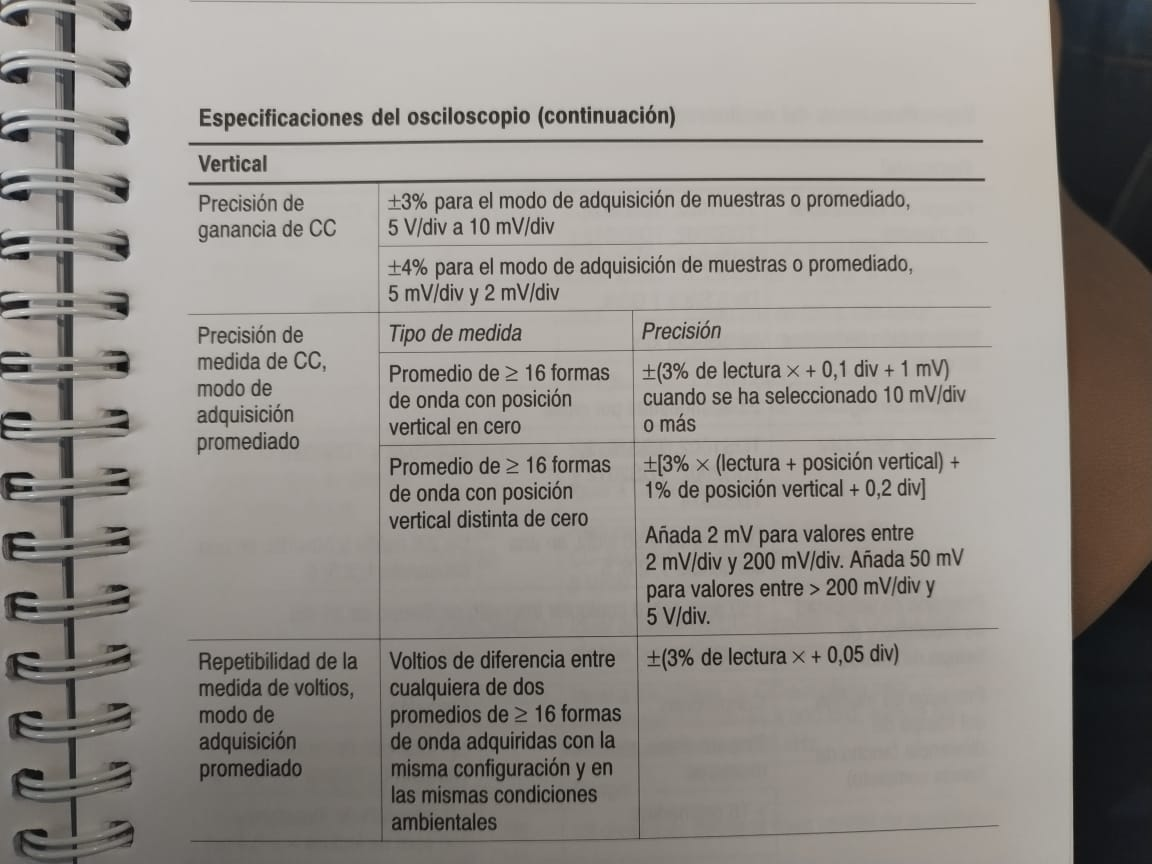
\includegraphics[scale=0.2]{Precisionosc.jpg} \\
    \hline 
    Temperatura de Servicio  & 0°C a 50°C \\
    \hline 
    Temperatura de Almacenamiento & -40 a 71 °C \\
    \hline 
    Error Estatico & No aplica \\
    \hline 
    Zona Muerta  & No aplica \\
    \hline 
    Supresión de cero & No aplica \\
    \hline 
    Vida util de la batería & 10 años \\
    \hline


\end{tabular}
\end{center}


\section{Observaciones y Conclusiones}

\subsection{Observaciones}
\indicacion{
    Elaborar las observaciones correspondientes.
}

\subsection{Conclusiones Personales}
\indicacion{
    Realizar las conclusiones correspondientes de forma personal anexando usos y aplicaciones de lo aprendido.
}


  
%\nocite{*}

%\printbibliography[
%heading=bibintoc,
%title={ . }
%]
    \end{document}